\documentclass[a4paper, 12pt]{article}
\usepackage[margin=1.25in]{geometry}
\usepackage{graphicx}
\usepackage{fontspec}
\usepackage[hidelinks]{hyperref}
\usepackage{bookmark}
\usepackage{booktabs}
\usepackage{xcolor}
\usepackage{eso-pic}
\usepackage{anyfontsize}
\usepackage{titlesec}
\usepackage{titletoc}
\usepackage{afterpage}
\usepackage{framed,color,verbatim}
\usepackage[norsk]{babel}
\usepackage{pgf-umlcd}
\usepackage{dirtree}
\usepackage{listings}
 \usepackage[charter]{mathdesign}

\definecolor{USNBlue}{rgb}{0.275,0.275,0.647}
\definecolor{shadecolor}{rgb}{.2, .2, .2}

\setsansfont{Ubuntu}[
    Path=./res/Ubuntu/,
    Extension = .ttf,
    UprightFont=*-Light,
    BoldFont=*-Regular,
    ItalicFont=*-LightItalic,
    BoldItalicFont=*-Italic
    ]

\renewcommand{\familydefault}{\sfdefault}

\lstset{language=C++,
        backgroundcolor=\color{shadecolor},
        keepspaces=true,   
        breaklines=true,
        showstringspaces=false,
        basicstyle=\ttfamily\color{white},
        keywordstyle=\color{cyan}\ttfamily,
        stringstyle=\color{yellow}\ttfamily,
        commentstyle=\color{teal}\ttfamily,
        morecomment=[l][\color{magenta}]{\#}
}

\newcommand\BackgroundPic{%
\put(0,0){%
\parbox[b][\paperheight]{\paperwidth}{%
\vfill
\centering
\includegraphics[scale=0.55, keepaspectratio]{res/background.jpg}%
\vfill
}}}

\newenvironment{myquote}{%
\begin{center}
  \begin{minipage}{0.9\textwidth}
    \small
}{%
  \end{minipage}
\end{center}
}

\newenvironment{code}%
   {%
      \snugshade%
      \verbatim}%
   {%
      \endverbatim%
      \endsnugshade%
   }

\begin{document}
\pagecolor{USNBlue}\afterpage{\nopagecolor}
\begin{titlepage}
    \centering
    {\color{white}%
    \vspace*{\fill}

    {\fontsize{35}{40}\bfseries
    \selectfont Operativsystemer\\[0.5ex]
    \fontsize{50}{60}\bfseries
    \selectfont Ringbuffer}

    \vspace*{0.5cm}
    {\fontsize{25}{25}\selectfont TSD2110-1 | Ruben Sørensen}

    \vspace*{0.25cm}
    \normalsize \today

    \vspace*{\fill}
    \includegraphics[]{res/USN.png}
    }
    \end{titlepage}
    \clearpage

    \tableofcontents
    \clearpage

    \section{Introduksjon}
    Denne obligen består av å implementere et ringbuffer i C++, og opprette tre \textit{barn}-prosesser: En prosess som leser input fra brukerens tastatur og legger dette til i ringbufferet, en prosess som legger data fra en string inn i ringbufferet og en prosess som henter ut data fra ringbufferet og printer det til \textit{standard output}.
    \subsection{Ringbuffer}
    Et ringbuffer er en sirkulær datastruktur. Størrelsen på bufferet er basert på to indekser, \textit{start} og \textit{end}. Disse kan også tenkes på som \textit{read} og \textit{write} indekser, fordi vi legger alltid til data bakerst i bufferet, og henter ut data fremst. Ringbufferet er altså en first in first out (FIFO) datastruktur, lignende en \textit{queue}. Fig. \ref{fig:ringbuffer} viser et ringbuffer visualisert. Denne figuren er hentet fra {\color{cyan}\href{https://en.wikipedia.org/wiki/Circular_buffer}{ringbuffer-artikkelen på wikipedia}}.

    \begin{figure}[h!]
      \centering
      \includegraphics[scale=0.2]{res/ringbuffer.png}
      \caption{Ringbuffer}
      \label{fig:ringbuffer}
    \end{figure}

    \subsection{Prosesser}
    De fleste programmer vi har skrevet har kjørt en prosess, dette er generet \textit{main}-funksjonen i koden. I denne oppgaven må vi kjøre flere parallelle prosesser som vil være såkalte \textit{barne-prosesser} av hovedprosessen. Dette gjør vi ved å starte tråder fra koden. Trådene mottar en funksjon som de utfører parallelt med hovedtråden. En utfordring vi møter når vi parallelliserer applikasjoner og prosessene opererer på samme minne, er at prossessene ikke automatisk blir synkronisert. Vi må derfor bruke teknikker for å hindre at prosessene kolliderer og prøver å utføre operasjoner på samme minne samtidig. Disse teknikkene har samlebetegnelsen synkronisering.

    \section{Plan}
    \subsection{Klasse: Ringbuffer}
    Ringbufferet blir implementert som en klasse. Klassen inneholder dataen som er i bufferet i en medlemsvariabel et array på en gitt størrelse. Fig. \ref{fig:class_diagram} viser et klassediagram for et enkelt ringbuffer. Min implementasjon inneholder litt flere medlemmer, fordi jeg gir ringbufferet selv ansvaret for synkronisering av tråder. Jeg synes selv dette \underline{ikke} er en god løsning, jeg tar derfor for meg hva jeg ville gjort annerledes om jeg skulle implementere dette på nytt i seksjon \ref{sec:forbedring}.

    \begin{figure}[h!]
      \centering
      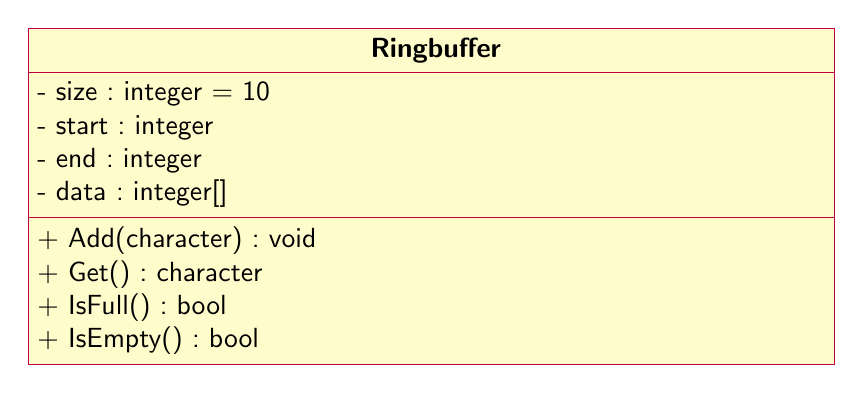
\begin{tikzpicture}
        \begin{class}[text width=10cm]{ Ringbuffer }{0,0}
          \attribute{- size : integer = 10}
          \attribute{- start : integer}
          \attribute{- end : integer}
          \attribute{- data : integer[]}
          \operation{+ Add(character) : void}
          \operation{+ Get() : character}
          \operation{+ IsFull() : bool}
          \operation{+ IsEmpty() : bool}
        \end{class}
      \end{tikzpicture}
      \caption{Klasse-diagram av ringbuffer}
      \label{fig:class_diagram}
    \end{figure}

    \subsection{Barneprosesser}
    Programmet består av fire prosesser: \textit{Parent-prosessen}, eller main prosessen, og dens tre barnprosesser. De tre barnprosessene kjører alle parallelt og har ansvar for forskjellige operasjoner. En har ansvar for å lese inn input fra brukerens tastatur og legge inputet til i ringbufferet. Denne funksjonen kaller jeg \textbf{KeyboardReader}. En har ansvar for å gå gjennom en string og legge alle characters til i ringbufferet, med et gitt intervall. Jeg kaller denne funksjonen \textbf{StringReader}. Den siste prosessen har ansvar for å hente ut alle verdier i ringbufferet, og printe disse til standard output. Denne siste funksjonen kaller jeg \textbf{BufferReader}. Disse tre funksjonene skal altså kjøres på hver sin tråd, men skal alle operere på samme ringbuffer.

    \subsection{Synkronisering}
    Siden alle prosesser opererer på samme ringbuffer, vil ringbufferet være definert som et delt minne. Når vi har delt minne mellom prosesser, må vi på et eller annet vis synkronisere disse prosessene. Siden prosesser kjører parallelt, kan ikke vi som programmere bestemme akkurat når noe skjer fordi operativsystemet hopper litt fram og tilbake mellom prosesser. Det vi \underline{kan} gjøre, er å definere såkalte \textit{kritiske regioner}. Når vi definerer en region som kritisk, spesifikt ved å bruke mutex, mutual exclusion, får bare en tråd operere på den regionen om gangen. 
    
    Oppgaveteksten ber oss opprette et semaforsett. I min implementasjon simulerer jeg operasjonen til en semafor ved å bruke mutex og condition variabler: Når en tråd vil legge til en verdi i bufferet, vil det først bli sjekket om bufferet er fullt. Hvis det er fullt, blir tråden satt i en wait state frem til den mottar et klarsignal fra en annen prosess om at det er ledig plass. Etter data har blitt lagt til i bufferet, sendes det ut et klarsignal til en tråd som venter på at data blir lagt til. Å hente ut data har en motsatt test: Hvis bufferet ikke inneholder data, blir tråden satt i en wait state frem til den mottar et klarsignal om at data har blitt lagt til. Etter data er hentet ut, blir det sendt ut et klarsignal om at det er ledig plass i bufferet til en tråd som venter på plass. Denne synkronisering skjer i min implementasjon inni Add og Get metodene til ringbuffer klassen.

    \section{Kode}
    Kildekoden ligger tilgjengelig på min {\color{cyan}\href{https://github.com/rubensorensen/ringbuffer}{Github bruker}}, men er også lagt til i denne seksjonen.

    \subsection{Filstruktur}
    Prosjektet har følgende filstruktur:
    \dirtree{%
    .0 .
    .1 include/.
    .2 readers.hpp.
    .2 ringbuffer.hpp.
    .1 src/.
    .2 main.cpp.
    .2 ringbuffer.cpp.
    .1 makefile.
    }

    \newgeometry{left=0.5cm, right=0.5cm, top=0.5cm, bottom=0.5cm}
    \subsection{Filer}
    \subsubsection{include/ringbuffer.hpp}
    \lstinputlisting[language=C++]{../include/ringbuffer.hpp}
    \clearpage
    \subsubsection{src/ringbuffer.cpp}
    \lstinputlisting[language=C++]{../src/ringbuffer.cpp}
    \clearpage
    \subsubsection{include/readers.hpp}
    \lstinputlisting[language=C++]{../include/readers.hpp}
    \clearpage
    \subsubsection{src/main.cpp}
    \lstinputlisting[language=C++]{../src/main.cpp}
    \restoregeometry

    \section{Forbedringspotensiale} \label{sec:forbedring}
    Jeg har lært mye av å implementere ringbuffer og synkronisere prosesser som bruker det. Hvis jeg skulle gjort det igjen fra bunnen av er det flere ting jeg ville gjort annerledes. Jeg liker ikke arkitekturen jeg har bygget hvor ringbufferet er selv ansvarlig for synkronisering. Jeg vil mye heller at ringbufferet bare er et ringbuffer med enkle metoder for å legge til og hente ut data. Jeg vil heller ha dedikerte klasser som håndterer prosesser og synkroniserer disse. Jeg ville altså implementert en \textit{master} klasse som har et ringbuffer som medlem. Denne-klassen vil også holde på en rekke \textit{worker} objekter i en vector, som holder på en funksjonspeker, som er funksjonen de skal utføre. Når Run() metoden til worker klassen blir kalt, vil den starte en ny tråd og utføre funksjonen sin på Master sitt ringbuffer. Masteren står ansvarlig for å sende ut klarsignaler, etterhvert som worker-klassene sender sine \textit{done} signaler.

    En annen endring jeg ville gjort var å utforske muligheten for å bruke C++ sin innebygde semafor klasse, for å unngå å manuelt "simulere" en semafor v.h.a. condition variabler og mutexer. Jeg er også interesert i å prøve å implementere min egen semafor klasse.

    Jeg har dessverre ikke tid til å utforske disse endringene innenfor tidsrammene til denne oppgaven, men dette er defintivt noe jeg kommer til å eksperimentere med senere.
    
\end{document}
